\documentclass[prl,twocolumn]{revtex4-1}
\usepackage{graphicx}
\usepackage{amsmath}
\usepackage{hyperref}
\usepackage{booktabs}
\usepackage{xcolor}

\usepackage{siunitx}

\setlength{\tabcolsep}{10pt}

\newenvironment{sistema}%
  {\left\lbrace\begin{array}{@{}l@{}}}%
  {\end{array}\right.}


\usepackage{pgfplots}
\usepgfplotslibrary{external}
\usepgfplotslibrary{groupplots}
\usepgfplotslibrary{units}
\usepgflibrary{decorations.shapes, decorations.fractals}
\usetikzlibrary{positioning, plotmarks, matrix, fit, shapes.geometric}
\tikzexternalize
%\tikzset{external/force remake}
\tikzset{every mark/.append style={scale=0.8}}
\pgfplotsset{every axis/.append style={small}}
\usepackage{pgfplots}
\pgfplotsset{compat=1.9}
\usepgfplotslibrary{groupplots}
\usepgfplotslibrary{external}
\tikzexternalize
\tikzsetexternalprefix{figs/}

\begin{document}
\tikzset{external/force remake=false}

\begin{figure*}
	%\tikzset{external/force remake}
	\tikzsetnextfilename{cell_vs_cap}
	\begin{tikzpicture}[
		pic3d/.style={inner sep=0}, %
		lab/.style={below right, text height=0.8em, text depth=0.2em, font=\Large\bfseries},%
		]%
		%box
		\draw[every node/.style={draw, inner sep=0, minimum width=0.01\textwidth, minimum height=0.12\textwidth, anchor=south west}] 
			node (Rrightwall) at (0, 0) {}
			node (Rleftwall) at (0.2\textwidth, 0) {}
			[every node/.append style={minimum height=0.06\textwidth}]
			node (Crightwall) at (0, 0.13\textwidth) {}
			node (Cleftwall) at (Crightwall.south -| Rleftwall.west) {}
			(Crightwall.north west) +(0,0.005\textwidth) rectangle (Cleftwall.north east);
			
	
		%filtre
		\foreach \x / \y in {0/0.23, 0.27/0.48, 0.52/0.73, 0.77/1}
			\fill[gray] ($(Rrightwall.north west)!\x!(Rleftwall.north east)$) rectangle ($(Crightwall.south west)!\y!(Cleftwall.south east)$);
		
		
		%laser
		\node[fill, green, semitransparent, isosceles triangle, anchor=apex, shape border rotate=-90, minimum width=0.08\textwidth, inner sep=0,  isosceles triangle apex angle=75] at ($(Crightwall.north east)!0.4!(Cleftwall.south west)$) (laser) {};
		
		%lens
		\filldraw[lightgray] (laser.right corner) arc[start angle=180,delta angle=180,x radius=0.04\textwidth, y radius=0.01\textwidth] --cycle;
		%colloids
		\begin{scope}[radius=0.008\textwidth, ball color=red!80]
			\shade(0.08\textwidth, 0.175\textwidth) circle;
			\shade(0.11\textwidth, 0.16\textwidth) circle;
			\shade(0.05\textwidth, 0.15\textwidth) circle;
			\shade(0.03\textwidth, 0.18\textwidth) circle;
			\shade(0.14\textwidth, 0.14\textwidth) circle;
			\shade(0.16\textwidth, 0.165\textwidth) circle;
		\end{scope}
		
		%polymers
		\foreach \x / \y in {0.06/0.1745, 0.17/0.1345, 0.172/0.14, 0.145/0.16, 0.19/0.18, 0.09/0.14, 0.03/0.15} 
			\draw[%
			gray, decoration={coil, segment length=0.0025\textwidth, amplitude=0.0025\textwidth},
			] (\x\textwidth, \y\textwidth)
			decorate{++(-0.0025\textwidth,-0.0025\textwidth) -- ++(0.0045\textwidth,0.0045\textwidth) -- ++(0,-0.0045\textwidth) -- ++(-0.005\textwidth,+0.005\textwidth) };
		
		
		%salt
		\begin{axis}[
			at={($(Rrightwall.south east)+(0.75,0.75)$)},
			width=0.19\textwidth-2*0.75,
			height=0.115\textwidth,
			axis lines=none,
			scale only axis,
			xmin=-1, xmax=1,ymin=0,ymax=1,
			]
			\addplot [blue, only marks, mark=*, samples=1000, mark size=0.75]
    {rand^2};
		\end{axis}
		
		%arrows
		\foreach \x in {0.25,0.5,0.75}
			\draw[blue!20,->, line width=0.005\textwidth] ++($(Rrightwall.south west)!\x!(Rleftwall.south east)$) +(0, 0.08\textwidth) -- +(0, 0.11\textwidth);
		
		
		%labels
		\begin{scope}[right, font=\footnotesize]
			\node[above right=0 of Rleftwall.south east] (Reservoir) {Reservoir};
			\node[anchor=north west] at (laser.lower side-|Reservoir.west) {Objective lens};
			\node at (Cleftwall-|Reservoir.west) (oc) {Observation cell};
			\node[anchor=base west] at (Rleftwall.north-|Reservoir.west){Filter};
			\node[above right,blue] at (Rleftwall.east-|Reservoir.west) {Salt diffusion};
			%\node[above right] at (0.21\textwidth, 0) {Reservoir};
		\end{scope}
			
		\node[inner sep=0pt,thick,fit=(Rrightwall) (oc) (laser)
		] (cellsketch) {};
		\node[lab, below right=0, inner sep=0] at (cellsketch.north west) {a};
		
		%%%%Capillary vs Reservoir Cell%%%
		\node[inner sep=0, below right=0 and 1em of cellsketch.north east] (ResSnapshot) {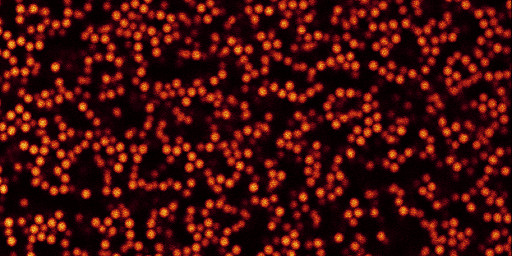
\includegraphics[width=0.2\textwidth]{Res362A_scan2Snapshot1.jpg}};
		\node[inner sep=0, above right=0 and 1em of cellsketch.south east] (CapSnapshot) {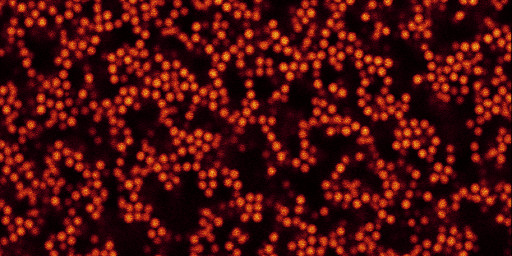
\includegraphics[width=0.2\textwidth]{Cap362_Snapshot1.jpg}};
		\node[lab,white] at (ResSnapshot.north west) {b};
		\node[lab,white] at (CapSnapshot.north west) {c};
		
		%%%%Phase diagram%%%%
		
		\begin{axis}[%
			at={($(cellsketch.north west)+(\textwidth,0)$)}, anchor=outer north east,%
			name={phasediag},%
			width=0.425\textwidth, height=0.3\textwidth,%
			xmin=0, xmax=40, xlabel={$\phi$}, x unit={\%},
			ymin=0.08, ymax=3.5, ylabel={$c_p$}, y unit={\si{\gram\per\litre}},%
			%ytick={0.1,0.2,0.3,0.4,0.5,0.6,0.7,0.8,0.9,1,2}, yticklabels={0.1,0.2,,,0.5,,,,,1,2},%
			legend pos=north east,%
			legend style={font=\footnotesize},%
			only marks,%
			]%
			\addplot[sharp plot, no marks] table [x expr=100*\thisrowno{0}, y index=1] {gasliquid_sg.phd};
			%\addplot[sharp plot, no marks, dashed] table [x expr=100*\thisrowno{0}, y index=1] {gasliquid_bg.phd};
			%\addplot[sharp plot, no marks, dotted] table [x expr=100*\thisrowno{0}, y index=1] {fluidsolid_f.phd};
			%\addplot+[forget plot] table [x index=1,y index=2] {phase_diag_capillary.csv};
			\addplot table [x index=1,y index=2] {phase_diag_gel.csv};
			\addplot table [x index=1,y index=2] {phase_diag_fluid.csv};
			\addplot table [x index=1,y index=2] {phase_diag_clusters.csv};
			\legend{spinodal, gel, fluid, clusters};
			\node[circle, draw, gray] at (axis cs:7.4, 0.98) (155C) {};
			\node[draw, gray] at (axis cs:25.7, 1.43) (Cap1) {};
		\end{axis}
		\node[lab] at (phasediag.outer north west) {d};
		
		%scale bar
		\draw[ultra thick] node[anchor=south east, inner xsep=0] (sb) at (CapSnapshot.south east |- phasediag.outer south)  {\SI{50}{\micro\metre}} (sb.north east) -- +(-0.069\textwidth,0);
	\end{tikzpicture}
	\caption{\textbf{Reservoir cell} \textbf{a} Sketch of our experimental setup. The observation cell contains initially colloids, polymer and no salt. \textbf{b} Confocal picture of a gel formed in situ ($\phi=25.5~\%$, $c_p=\SI{1.4}{\gram\per\litre}$), \SI{1}{\hour} after gelation. \textbf{c} Confocal picture of a gel at the same state point formed ex situ, \SI{1}{\hour} after shear melting. \textbf{d} Phase diagram obtained in reservoir cell. Spinodal line is obtained from free volume theory.}
	\label{fig:cell_vs_cap}
\end{figure*}

\begin{figure}
	%\tikzset{external/force remake}
	\tikzsetnextfilename{hydro}
	\begin{tikzpicture}[lab/.style={below right, text height=0.8em, text depth=0.2em, font=\Large\bfseries}]
		\begin{groupplot}[%
			group style={
				group name=g, group size=2 by 1,
				horizontal sep=4em,
				},
			width=0.5\columnwidth+1em,%
			height=0.5\columnwidth,
			ylabel absolute, every axis y label/.append style={anchor=base, yshift=-1.5em}
			]
			\nextgroupplot[
			xlabel={$t/\tau_B$}, xmin=0, xmax=20,%
			ylabel={$R_g/\sigma$},
			]%
			\addplot table [x expr=\thisrowno{0}*6, y expr=\thisrowno{1}]{cluster_Rg_dynamics_N3.csv} node[pos=0, above right] {all};
			\addplot table [x expr=\thisrowno{0}*6, y expr=\thisrowno{2}]{cluster_Rg_dynamics_N3.csv} node[pos=0, right] {most elongated};
			\addplot table [x expr=\thisrowno{0}*6, y expr=\thisrowno{3}]{cluster_Rg_dynamics_N3.csv} node[pos=0, above right] {least elongated};
			%\legend{All triplets, Most elongated 20\%, Most compact 20\%};
			
		\nextgroupplot[
			width=0.5\columnwidth,
			xlabel={$t/\tau_B$}, xmin=0, xmax=400,
			ymin=0, ymax=1, ylabel={aspect ratio},
			only marks,]
		\addplot table[x expr=\thisrowno{0}*6-19] {172A_1206_percolation.aspect} node[below left] {$\lambda_3/\lambda_1$};
		\addplot table[x expr=\thisrowno{0}*6-19, y index=3] {172A_1206_percolation.aspect} node[above left] {$\lambda_2/\lambda_1$};
	\end{groupplot}
		
	\begin{axis}[
		name=hist,
		anchor=above north west,
		at={(g c1r1.below south west)},
		xlabel={angle (degree)}, xmin=0,xmax=180,%
		ylabel={probability (degree${}^{-2}$)}, ymin=0,
		no markers,%
		width=\columnwidth,
		height=0.6\columnwidth,
		ylabel absolute, every axis y label/.append style={anchor=base, yshift=-1.5em}
		]
			\addplot+[gray!50, fill=gray!50, area legend] file {all.angles} \closedcycle;
			\addplot file {new.angles};
			\addplot+[blue] file {alone.angles};
			\legend{existing, future, isolated};
			
			%sketch future
			\fill[radius=0.6em, red!50] (axis cs:20,0.02) circle[] +(0,1.2em) circle[] ++(1.2em,0) circle[] +(-120:1.2em) circle[];
			\draw[ultra thick] (axis cs:20,0.02) -- ++(1.2em,0) -- +(-120:1.2em);
			\draw[thick, dotted] (axis cs:20,0.02) +(1.2em,0) -- +(0,1.2em);
			
			%sketch alone
			\fill[radius=0.6em, blue!50] (axis cs:90,0.04) circle[] +(-1.2em,0) circle[] +(-120:1.2em) circle[] +(30:1.5em) circle[];
			\draw[ultra thick] (axis cs:90,0.04) -- +(-1.2em,0) (axis cs:90,0.04)-- +(-120:1.2em);
			\draw[thick, dotted] (axis cs:90,0.04) -- +(30:1.5em);
		\end{axis}
			
		\node[lab] at (g c1r1.outer north west) {a};
		\node[lab] at (g c2r1.outer north west) {b};
		\node[lab] at (hist.outer north west) {c};
	\end{tikzpicture}
	\caption{\textbf{Hydrodynamics} \textbf{a} Evolution of triplet radii of gyration in a non percolating sample ($\phi=4~\%$, $c_p=\SI{1}{\gram\per\litre}$). The characteristic time to reach the stable compact cluster is much longer than the Brownian time. \textbf{b} Evolution of the aspect ratios of clusters of 4 particles and more in a percolating sample ($\phi=8~\%$, $c_p=\SI{1.5}{\gram\per\litre}$) \textbf{c} Bond angle distribution relative to existing bonds (gray), to a future bond (red) or to a future bond involving an isolated particle (blue). Future bonds are shifted to smaller angles, whereas gas adsorption takes place from larger angles. Insets sketch both cases, with present bonds drawn thick and future bonds drawn dotted.}
	\label{fig:hydro}
\end{figure}
%\tikzset{external/force remake=false}




\begin{figure}
	%\tikzset{external/force remake}
	\tikzsetnextfilename{wholeprocess}
	\begin{tikzpicture}[
		lab/.style={below right, text height=0.8em, text depth=0.2em, font=\Large\bfseries},%
		]
	\pgfplotscreateplotcyclelist{earthy}{%
	black,
	red!40!black,
	red!60!black,
	red!80!black,
	red,
	red!80!yellow,
	red!60!yellow,
	red!40!yellow,
	}
	\begin{groupplot}[
	group style={
			group name=g, group size=2 by 1,
			horizontal sep=4em,
			},
		width=0.5\columnwidth+1em,%
		height=10\baselineskip,%
		ylabel absolute, every axis y label/.append style={anchor=base, yshift=-1.5em}
		]
%		\nextgroupplot[
%			xlabel={time (min)}, xmin=0,
%			ymin=0, ymax=1, ylabel={aspect ratio},
%			only marks,]
%		\addplot table {155C_percolation_1645.aspect} node[below left] {$\lambda_3/\lambda_1$};
%		\addplot table[y index=3] {155C_percolation_1645.aspect} node[above left] {$\lambda_2/\lambda_1$};
		\nextgroupplot[
			xlabel=$q^2\sigma^2$, xmin=0,
			ylabel=$A\tau_B/q^2\sigma^2$, ymin=0, ymax=0.2, ytick={0,0.1,0.2},
			]
		\addplot[only marks] table[x expr=\thisrowno{0}^2, y expr=\thisrowno{1}/\thisrowno{0}^2] {155C.growth};
		\addplot[no marks, red, domain=1.6:7] {1.5*(1-0.115*x)/(1+3.62*x)}; 
		
		\nextgroupplot[
			xmode=log, ymode=log,
			xlabel={$(t-t_0)/\tau_B$}, xmin=1,
			ylabel=$\langle q\rangle\sigma$, ymin=0.6,
			ytick={0.6,0.8,1,1.2,1.6,2}, yticklabels={0.6, 0.8,1,1.2,1.6, 2},
			]
		\addplot[only marks] table[x expr=6*(\thisrowno{0}-5)]{155C.qmax};
		\addplot+[red, no marks, domain=20:200] {4*x^(-1/3)} node[midway, below left]{$-1/3$};
	\end{groupplot}

	\begin{axis}[name=Sq,
		anchor=below south west,
		at={(g c1r1.above north west)},
		xmin=0, xmax=13, ymin=0,
		xlabel=$q\sigma$, ylabel=$S(q)$,
		ylabel absolute, every axis y label/.append style={anchor=base, yshift=-1.5em},
		scale only axis,
		width=\columnwidth-3.5em,
		height=6\baselineskip,
		no marks, cycle list name=earthy]
		\foreach \ii in {1,2,...,7}
			\addplot table[y index=\ii] {155C_every150s.Sqs};
		\draw[<-] (axis cs:3.1,3.3) -- +(45:1em) node[right]{Wigner};
		\draw[<-,red!80!black] (axis cs:6.5,1.9) -- +(45:1em) node[right]{Hard sphere};
		\draw[<-,red!60!yellow] (axis cs:0.8,7.5) -- +(0:1em) node[right]{Gelation};
	\end{axis}

	
	\matrix[
		matrix of nodes, inner sep=0, column sep=0.01\textwidth, row sep=0.5em,
		matrix anchor=south west,
		%at={($(g c1r1.outer north west)$)},
		at={($(Sq.outer north west)+(0,1em)$)},
		] (m){
		\SI{0}{\minute} & \SI{5}{\minute} \\
		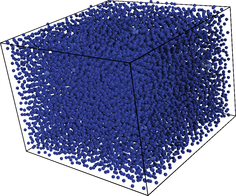
\includegraphics[width=0.48\columnwidth]{155C_percolation_1645_p2size_t024s.png}&
		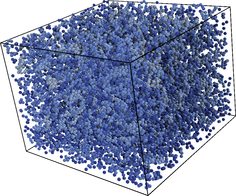
\includegraphics[width=0.48\columnwidth]{155C_percolation_1645_p2size_t044s.png}\\
		\SI{15}{\minute} & \SI{25}{\minute}\\
		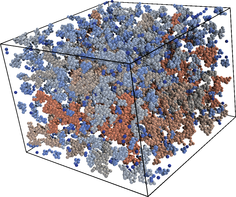
\includegraphics[width=0.48\columnwidth]{155C_percolation_1645_p2size_t084s.png} &
		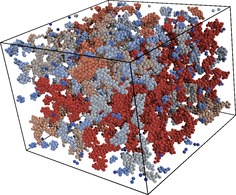
\includegraphics[width=0.48\columnwidth]{155C_1715_ageing_p2size_t00s.png}\\
		 \SI{35}{\minute} & \SI{45}{\minute}\\
		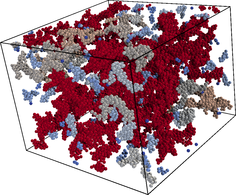
\includegraphics[width=0.48\columnwidth]{155C_1715_ageing_p2size_t20s.png}&
		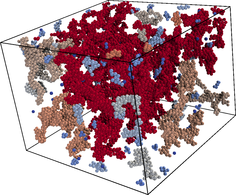
\includegraphics[width=0.48\columnwidth]{155C_1715_ageing_p2size_t40s.png}\\
		};
	\node[lab] at (m.north west) {a};
	\node[lab] at (Sq.outer north west) {b};
	\node[lab] at (g c1r1.outer north west) {c};
	\node[lab] at (g c2r1.outer north west) {d};
	\end{tikzpicture}
\caption{\textbf{Gelation observed in-situ} in a typical sample ($\phi=7.5~\%$, $c_p=\SI{1}{\gram\per\litre}$). Origin of time is the last frame before melting of Wigner crystal. \textbf{a} Reconstruction of experimental coordinates coloured by the number of particles in clusters. \textbf{b} Structure factor evolution (a curve every \SI{150}{\second}). \textbf{c} Cahn plot of the initial growth rate $A(q)$. The line is a fit by Eq. XXX with $\xi=0.11\sigma$ and $\xi_{ve}=3.6\sigma$. \textbf{d} Growth of the characteristic wave number.}
\label{fig:wholeprocess}
\end{figure}

\begin{figure*}
\tikzset{external/force remake}
\tikzsetnextfilename{breaking}
\begin{tikzpicture}[
	lab/.style={below right, text height=0.8em, text depth=0.2em, font=\Large\bfseries},%
	]
	\begin{groupplot}[
	group style={
			group name=g, group size=1 by 2,
			%horizontal sep=4em,
			},
		width=0.25\textwidth,%
		height=8\baselineskip,%
		ylabel absolute, every axis y label/.append style={anchor=base, yshift=-1.5em}
		]
		\nextgroupplot[
			height=9\baselineskip,%
			xlabel=$L$, ylabel={count},
			xmode=log, ymode=log,
			ymin=1, xmin=1,
			clip marker paths=true,
			]
			\addplot+[only marks] file {172A_broken_length.hist};
			\addplot+[only marks] file {170A_broken_length.hist};
			\addplot+[only marks,mark=asterisk, black] file {150A_broken_length.hist};
			\addplot[domain=1:32, no marks] {1e6/x^3} node[midway, above right] {-3};
			\addplot[domain=1:10, no marks] {1e4/x^4} node[midway, below left] {-4};
			
		\nextgroupplot[
			xlabel=$q_2$, ylabel={$P(q_2)$ [\%]},
			xmin=0,xmax=1,
			ymin=0,
			no marks
			]
			\addplot table[y expr=\thisrowno{1}*100] {150A_broken_q2.proba};
			\addplot table[y expr=\thisrowno{1}*100] {150A_broken_q2_L2.proba};
	\end{groupplot}
	
	\matrix[
		matrix of nodes, inner sep=0, %column sep=0.01\textwidth, 
		row sep=0.5em,
		matrix anchor=north west,
		at={($(g c1r1.outer north east)+(-\textwidth,0)$)},
		] (m){
		\SI{0}{\minute} & \SI{16}{\minute} & \SI{22}{\minute} & \SI{30.5}{\minute} & \SI{31}{\minute} & \SI{90}{\minute} \\
		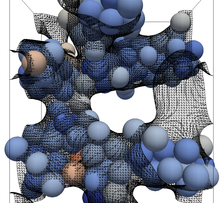
\includegraphics[width=0.13\textwidth]{breaking_particles_wireframe_t0000s.png}&
		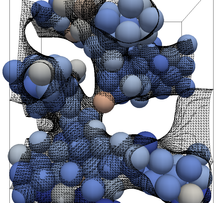
\includegraphics[width=0.13\textwidth]{breaking_particles_wireframe_t0032s.png}&
		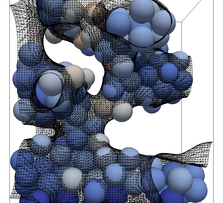
\includegraphics[width=0.13\textwidth]{breaking_particles_wireframe_t0043s.png}&
		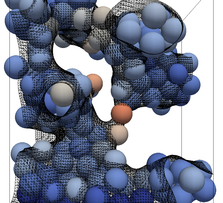
\includegraphics[width=0.13\textwidth]{breaking_particles_wireframe_t0061s.png}&
		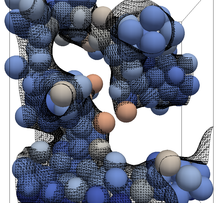
\includegraphics[width=0.13\textwidth]{breaking_particles_wireframe_t0062s.png}&
		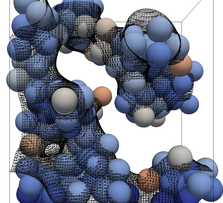
\includegraphics[width=0.13\textwidth]{breaking_particles_wireframe_t0180s.png}\\
		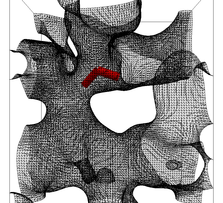
\includegraphics[width=0.13\textwidth]{breaking_wireframe_t0000s.png}&
		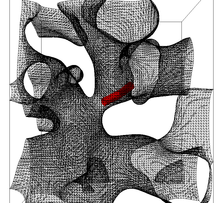
\includegraphics[width=0.13\textwidth]{breaking_wireframe_t0032s.png}&
		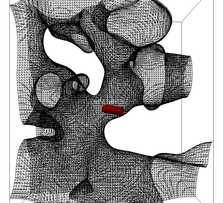
\includegraphics[width=0.13\textwidth]{breaking_wireframe_t0043s.png}&
		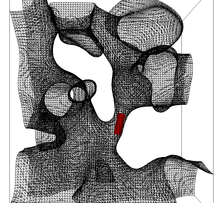
\includegraphics[width=0.13\textwidth]{breaking_wireframe_t0061s.png}&
		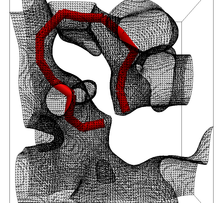
\includegraphics[width=0.13\textwidth]{breaking_wireframe_t0062s.png}&
		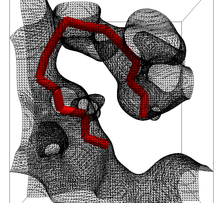
\includegraphics[width=0.13\textwidth]{breaking_wireframe_t0180s.png}\\
		};
	\node[lab] at (m.north west) {a};
	\node[lab] at (g c1r1.outer north west) {b};
	\node[lab] at (g c1r2.left of south west) {c};
\end{tikzpicture}
\caption{\textbf{Mechanical tension drives coarsening} 
\textbf{a} Reconstruction from experimental coordinates ($\phi=29~\%$, $c_p=\SI{0.7}{\gram\per\litre}$) of coarsening process geometry (top) and topology (bottom). Particles are drawn to scale and coloured by $q_2$ from blue (low) to red (high). The meshed surface is a Gaussian coarse-graining of the network pattern. The red line indicates the shortest on-graph path between the two particles of interest. 
\textbf{b} Number of bond breaking function of the future on-graph distance for three state points (after percolation): $\phi=8,\,18,\,29~\%$, $c_p=1.5,\,0.6,\,\SI{0.7}{\gram\per\litre}$ for \textcolor{blue}{$\bullet$}, \textcolor{red}{\tiny$\blacksquare$} and $*$ respectively.
\textbf{c} Probability for a bond to break during $3\tau_B$ function of bond-centred $q_2$ for all events (blue) and for events with $L>1$ (red) in the same sample as \textbf{a}.
}
\label{fig:breaking}
\end{figure*}

\end{document}